\documentclass{article}
\usepackage[margin=0.5in,includefoot]{geometry}% http://ctan.org/pkg/geometry
\usepackage{enumitem,fancyhdr,colortbl,graphicx}% http://ctan.org/pkg/{enumitem,fancyhdr,colortbl}
\usepackage{lastpage,lmodern,xcolor}% http://ctan.org/pkg/{lastpage,lmodern,xcolor}
\usepackage{multirow}
\usepackage[utf8]{inputenc}
\usepackage{tabularx}
\usepackage{verbatim}	%块注释
\usepackage{hyperref}%使用url
\usepackage[UTF8]{ctex}
\usepackage{mdwlist}
\usepackage{caption}
\usepackage{mathtools}
\usepackage{ragged2e}
\newlength{\outerbordwidth}
\pagestyle{empty}
\raggedbottom
\raggedright
%\usepackage{framed}
%\usepackage{times}
%\usepackage{tocloft}
%\usepackage{graphicx}

\renewcommand{\section}[1]{%
  \begin{tabular}{p{\dimexpr\linewidth-2\tabcolsep}}
    \cellcolor{black!10}\large\strut #1
  \end{tabular}%
}
\newcommand{\heading}[2][\relax]{\textbf{#2}\hfill#1\par\nobreak}
\newcommand{\pubheading}[1]{\par\bigskip\underline{\textbf{#1}}\par}
\newlist{subitems}{itemize}{1}
\setlist[subitems]{label={--},nosep}
\newlist{myreferences}{enumerate}{1}
\setlist[myreferences]{label={[\arabic*]},leftmargin=*}

\let\rmdefault\sfdefault% Default is sans serif
\setlength{\parindent}{0pt}% No indent
\pagestyle{fancy}% Fancy page styl
\fancyhf{}% Clear header/footer
\renewcommand{\headrulewidth}{0pt}% No header rule
\renewcommand{\footrulewidth}{.4pt}% Footer rule
\fancyfoot[L]{Curriculum Vitae - Xiaozhen Lu}% Left footer
\fancyfoot[R]{\thepage{} of \pageref{LastPage}}% Right footer
\begin{document}
	
% Header
%\begin{tabular}{@{}p{\linewidth}@{}}
%  \centering\LARGE Xiaozhen Lu \\
%  \centering\large \strut \\
%  \centering\large \strut  Associate Professor \\
%  \centering\large \strut Email: luxiaozhen@nuaa.edu.cn\\[\jot]
%  \hrule \mbox{}\\[\dimexpr-.4pt+\jot]
%  \small Research interests: wireless network security, reinforcement learning, blockchain\hfill  Email: luxiaozhen@nuaa.edu.cn
% % \small Email: luxiaozhen@nuaa.edu.cn\hfill Tel: +86-159-5191-9010
%\end{tabular}

\begin{tabular*}{7.5in}{l@{\extracolsep{\fill}}r}
  & \multirow{6}{*}{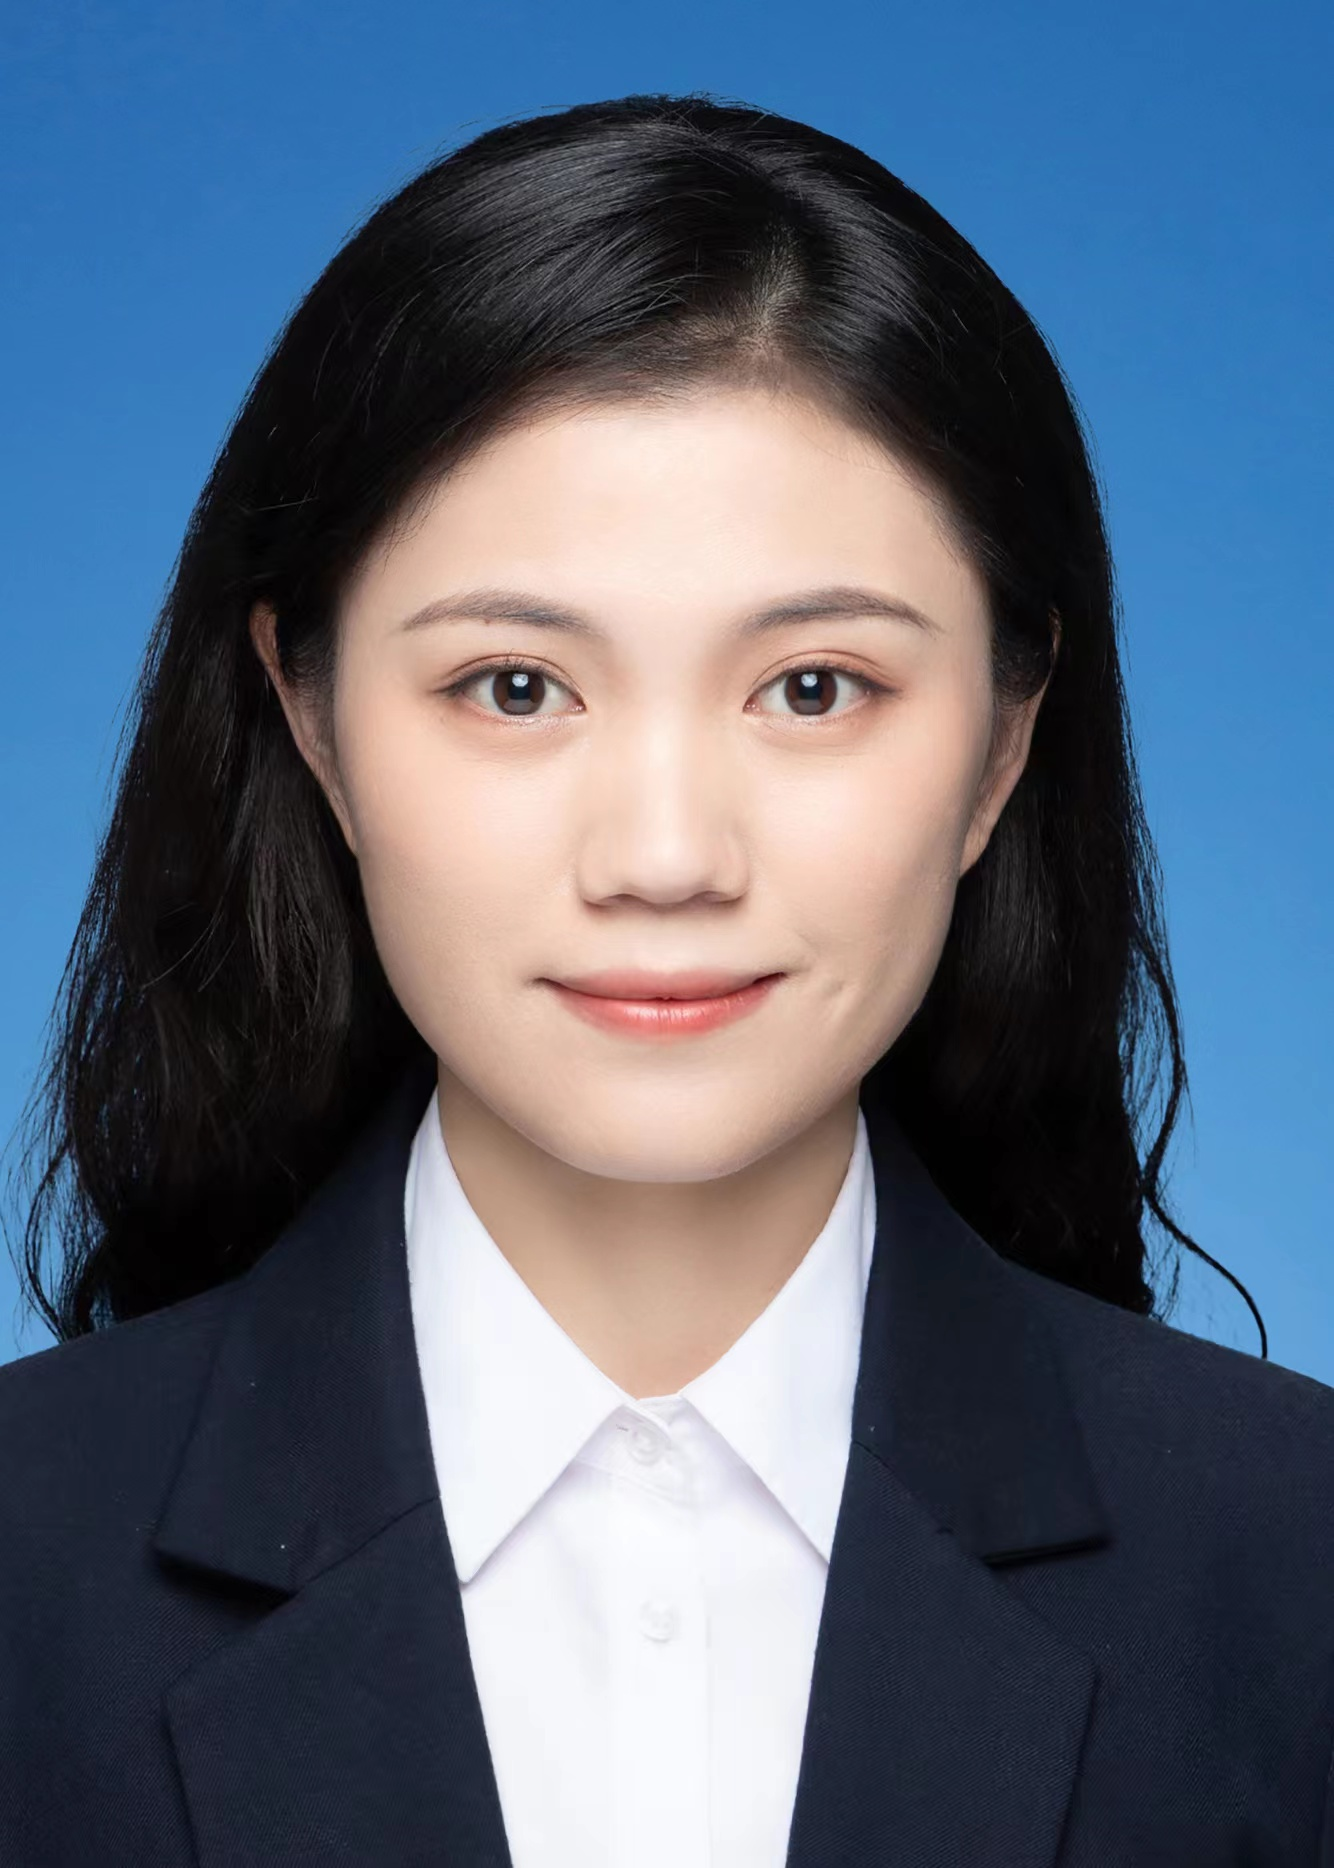
\includegraphics[scale=0.05]{Xiaozhen}}\\%  & \multirow{4}{*}{\includegraphics[scale=0.19]{iitmlogo}}
%-----------------------------------------------------------
  \textbf{\LARGE Xiaozhen Lu}  \\% $|$ EE10S0600
  \large Professor, Nanjing University of Aeronautics and Astronautics\\%Research Scholar
 \large  Email: luxiaozhen@nuaa.edu.cn, Tel: +86-159-5191-9010\\
  % \large \textbf{Research interests: low-altitude wireless secure communication, wireless access security, reinforcement learning}
  \large \textbf{Research interests:} low-altitude wireless secure communication, \\
  \large \hspace{3.7cm} wireless access security, reinforcement learning
\end{tabular*}
\vspace{3.5pt}

\renewcommand{\arraystretch}{1.5}% Spread titles out a tad...

\section{Education}
\begin{itemize}
  \item \heading[Sept. 2017 - Dec. 2021]{Ph.D., Communication and Information Systems}
    Xiamen University, Xiamen, China. Supervisor: Liang Xiao
    % \begin{subitems}
    %   \item Thesis title: Research on AI Aided Reliable Communications and Authentication for VANETs
    % \end{subitems}
  \item \heading[Sept. 2013 - Jun. 2017]{BE, Communication Engineering}
    Nanjing University of Posts and Telecommunications, Nanjing, China
\end{itemize}
\section{Work Experience}
\begin{itemize}
  \item \heading[Dec. 2021 - Mar. 2026]{Associate Professor}
    College of Computer Science and Technology, Nanjing University of Aeronautics and Astronautics, Nanjing, China
    \item \heading[Mar. 2026 - present]{Professor}
    College of Computer Science and Technology, Nanjing University of Aeronautics and Astronautics, Nanjing, China
\end{itemize}

\section{Honors and Awards}
\begin{justifying}
	\begin{myreferences}
		\item Liang Xiao, Di Wu, Minghui Min, and \textbf{Xiaozhen Lu}, Game theoretic study on smart IoT communication security based on reinforcement learning, \textcolor{blue}{Second Prize for Ministry of Education of Natural Science Award}, Jun. 2023.
		\item  \textbf{Xiaozhen Lu}, \textcolor{blue}{ACM China Rising Star Award}, Jul. 2023.
		\item \textbf{Xiaozhen Lu}, Research on AI Aided Reliable Communications and Authentication for VANETs, \textcolor{blue}{Excellent Doctoral Dissertation Award of Fujian Province}, Dec. 2023.
		\item \textbf{Xiaozhen Lu}, \textcolor{blue}{Jiangsu Young Scientists Support Program}, Oct. 2024.
		\item  Liang Xiao, \textbf{Xiaozhen Lu}, Tangwei Xu, Xiaoyue Wan, Wen Ji and Yanyong Zhang. Reinforcement learning based mobile offloading for edge computing against jamming and interference, \textcolor{blue}{Excellent Academic Paper Award of Natural Science in Fujian Province}, Dec. 2022.
		\item Jingfang Jie, \textbf{Xiaozhen Lu}, Tangwei Xu, Liang Xiao, and Yanyong Zhang. Robot relay for UAV communications against jamming: A reinforcement learning approach, \textcolor{blue}{Excellent Paper Award in the 14th China Conference on Internet of Things (Wireless Sensor Network)}, Sept. 2020.
		\item Zihan Lin, \textbf{Xiaozhen Lu}, Canhuang Dai, Geyi Sheng, and Liang Xiao. Reinforcement learning based UAV trajectory and power control against jamming, \textcolor{blue}{Best Student Paper Award in the 2nd International Conference on Machine Learning for Cyber Security}, Sept. 2019.
		\item \textbf{Xiaozhen Lu}, \textcolor{blue}{Changkong Star Award of Nanjing University of Aeronautics and Astronautics}, Aug. 2025.
		\item \textbf{Xiaozhen Lu}, \textcolor{blue}{Young Science and Technology Award of Jiangsu Information Technology Application Society}, Nov. 2025.
		\item \textbf{Xiaozhen Lu}, \textcolor{blue}{Excellent Instructor of the 27th China Robot and Artificial Intelligence Competition (Jiangsu Division)}, Jun. 2025.
		\item \textbf{Xiaozhen Lu}, \textcolor{blue}{IEEE International Conference on Computer and Communication Systems (ICCCS) Young Scientist Award}, Apr. 2026.
		\item \textbf{Xiaozhen Lu}, \textcolor{blue}{Young Elite Scientists Sponsorship Program by China Institute of Communications}, May 2026.
		\item \textbf{Xiaozhen Lu}, \textcolor{blue}{Second Prize of Xiamen Natural Science Award (2nd Contributor)}, Sept. 2026.
	\end{myreferences}
\end{justifying}

\section{Research Grants}
\begin{justifying}
\begin{itemize}
  \item \heading[Jan. 2026 - Dec. 2029]{National Natural Science Foundation of China, PI}
    \begin{subitems}
      \item Research on high-reliability wireless secure communication methods for low-altitude intelligent connected networks
    \end{subitems}
  \item \heading[Jan. 2023 - Dec. 2025]{National Natural Science Foundation of China, PI}
    \begin{subitems}
      \item Reinforcement learning for safety applications of VANETs
    \end{subitems}
  \item \heading[Jul. 2022 - Jun. 2025]{National Natural Science Foundation of Jiangsu Province, PI}
    \begin{subitems}
      \item Research on security policy optimization for Internet of vehicles with safe reinforcement learning
    \end{subitems}
  \item \heading[Jan. 2023 - Dec. 2026]{Joint Funds of the National Natural Science Foundation of China, CoPI}
    \begin{subitems}
      \item Key technology of hidden information detection network capable of cross-domain few-shot learning
    \end{subitems}
  \item \heading{Natural Science Foundation on Frontier Leading Technology Basic Research Project of Jiangsu, CoPI}
    \hfill{Oct. 2022 - Sep. 2027}
    \begin{subitems}
      \item Subproject 3: Fundamental research on 6G blockchain-enabled wireless networks in a zero-trust environment
    \end{subitems}
    \item \heading{Open research fund of National Mobile Communications Research Laboratory，Southeast University, PI}
    \hfill{Jan. 2026 - Dec. 2027}
    \begin{subitems}
      \item Federated reinforcement learning for secure resource scheduling of unmanned aerial vehicles
    \end{subitems}
    \item \heading[Jul. 2024 - Jun. 2025]{Open research of the Key Laboratory for Safety-critical Software Development and Verification, Ministry of Industry and Information Technology, PI}
    \begin{subitems}
      \item Secure communication mechanisms for internet of vehicles based on federated reinforcement learning
    \end{subitems}
  
\end{itemize}
\end{justifying}

\section{Publications}

\pubheading{Journal Papers}
\begin{justifying}
\begin{myreferences}
  \item \textbf{Xiaozhen Lu}, Liang Xiao, Yilin Xiao, Wei Wang, Nan Qi, and  Qian Wang, ``Risk-aware federated reinforcement learning-based secure IoV communications", \emph{IEEE Transactions on Mobile Computing}, vol. 23, no. 12, pp. 14656-14671, Dec. 2024. [CCF A]
  \item \textbf{Xiaozhen Lu}, Zihan Liu, Zhibo Liu, Yanling Bu*, and Huaiyu Dai, "Reinforcement learning-based efficient multi-exit neural networks against side-channel attacks", \emph{IEEE Transactions on Information Forensics and Security}, vol. 20, pp. 11830-11843, Nov. 2025. [CCF A]
  \item \textbf{Xiaozhen Lu}, Zhibo Liu, Yuhan Chen, Liang Xiao, Wei Wang, and Qihui Wu, ``Risk-aware reinforcement learning-based federated learning for IoV systems", \emph{IEEE Transactions on Mobile Computing}, vol. 23, no. 12, pp. 14672-14688, Dec. 2024. [CCF A]
  \item \textbf{Xiaozhen Lu}, Zihan Liu, Liang Xiao, and Huaiyu Dai, ``Reinforcement learning-based personalized differentially private federated learning", \emph{IEEE Transactions on Information Forensics and Security}, vol. 20, pp. 465-477, Dec. 2024. [CCF A]
  \item \textbf{Xiaozhen Lu}, Liang Xiao, Yilin Xiao, Zehui Xiong, Zhe Liu, Yanyong Zhang, and Weihua Zhuang, ``Blockchain-enabled secure offloading for VEC: A multi-agent reinforcement learning approach", \emph{IEEE Transactions on Dependable and Secure Computing}, vol. 22, no. 3, pp. 2978-2995, May 2025. [CCF A]
  \item \textbf{Xiaozhen Lu}, Lixin Liu, Zhibo Liu, Qihui Wu, and Liang Xiao, ``Blockchain-based intelligent trusted computational resource allocation for low-altitude networks", \emph{IEEE Transactions on Mobile Computing}, vol. 24, no. 10, pp. 10200-10213, Oct. 2025. [CCF A]
  \item  \textbf{Xiaozhen Lu}, Liang Xiao, Pengmin Li, Xiangyang Ji, Chenren Xu, Shui Yu, and Weihua Zhuang, ``Reinforcement learning based physical cross-layer security and privacy in 6G", \emph{IEEE Communications Surveys \& Tutorials}, vol. 25, no. 1, pp. 425-466, Firstquarter 2023. [\textcolor{blue}{IF: 33.840}]
  \item \textbf{Xiaozhen Lu}, Liang Xiao, Guohang Niu, Xiangyang Ji, and Qian Wang, ``Safe exploration in wireless security: A safe reinforcement learning algorithm with hierarchical structure", \emph{IEEE Transactions on Information Forensics and Security}, vol. 17, pp. 732-743, Feb. 2022. [\textcolor{blue}{Popular paper in IEEE Transactions on Information Forensics and Security}]
		\item \textbf{Xiaozhen Lu}, Jingfang Jie, Zihan Lin, Liang Xiao, Jin Li, and Yanyong Zhang, ``Reinforcement learning based energy efficient robot relay for unmanned aerial vehicles against smart jamming", \emph{Science China Information Sciences}, vol. 65, no. 112304, pp. 1-13, Jan. 2022.
		\item \textbf{Xiaozhen Lu}, Liang Xiao, Canhuang Dai, and Huaiyu Dai, ``UAV-aided cellular communications with deep reinforcement learning against jamming", \emph{IEEE Wireless Communications Magazine}, vol. 27, no. 4, pp. 48-53, Aug. 2020. [\textcolor{blue}{Popular paper in IEEE Wireless Communications Magazine}]
		\item \textbf{Xiaozhen Lu}, Liang Xiao, Tangwei Xu, Yifeng Zhao, Yuliang Tang, and Weihua Zhuang, ``Reinforcement learning based PHY authentication for VANETs", \emph{IEEE Transactions on Vehicular Technology}, vol. 69, no. 3, pp. 3068-3079, Mar. 2020. [\textcolor{blue}{IEEE ComSoc Best Readings in Physical-Layer Security: Foundations, Intelligent Designs and Implementations}]
        \item \textbf{Xiaozhen Lu}, Xingyu Xiao, Liang Xiao, Canhuang Dai, Mugen Peng, and H Vincent Poor, ``Reinforcement learning-based microgrid energy trading with a reduced power plant schedule", \emph{IEEE Internet of Things Journal}, vol. 6, no. 6, pp. 10728-10737, Dec. 2019.
		\item Liang Xiao, \textbf{Xiaozhen Lu}, Tangwei Xu, Weihua Zhuang, and Huaiyu Dai, ``Reinforcement learning based physical-layer authentication for controller area networks", \emph{IEEE Transactions on Information Forensics and Security}, vol. 16, pp. 2535-2547, Feb. 2021. [\textcolor{blue}{Popular paper in IEEE Transactions on Information Forensics and Security}]
		\item Liang Xiao, \textbf{Xiaozhen Lu}, Tangwei Xu, Xiaoyue Wan, Wen Ji, and Yanyong Zhang, ``Reinforcement learning-based mobile offloading for edge computing against jamming and interference", \emph{IEEE Transactions on Communications}, vol. 68, no. 10, pp. 6114-6126, Oct. 2020. [\textcolor{blue}{Popular paper in IEEE Transactions on Communications}]
		\item Liang Xiao, \textbf{Xiaozhen Lu}, Dongjin Xu, Yuliang Tang, Lei Wang, and Weihua Zhuang, ``UAV relay in VANETs against smart jamming with reinforcement learning", \emph{IEEE Transactions on Vehicular Technology}, vol. 67, no. 5, pp. 4087-4097, May 2018.
    \begin{subitems}
     	\item \textcolor{blue}{IEEE ComSoc Best Readings in UAV Assisted Wireless Networks}
        \item \textcolor{blue}{Popular paper in IEEE Transactions on Vehicular Technology}
        \item \textcolor{blue}{ESI Highly Cited Paper}
    \end{subitems}
    \item Liang Xiao, Xiaoyue Wan, \textbf{Xiaozhen Lu},Yanyong Zhang, and Di Wu, ``IoT security techniques based on machine learning: How do IoT devices use AI to enhance security?", \emph{IEEE Signal Processing Magazine}, vol. 35, no. 5, pp. 41-49, Sept. 2018.
    \begin{subitems}
        \item \textcolor{blue}{Popular paper in IEEE Signal Processing Magazine}
        \item \textcolor{blue}{ESI Highly Cited Paper}
    \end{subitems}
    \item Yilin Xiao, Liang Xiao, \textbf{Xiaozhen Lu}, Hailu Zhang, Shui Yu, and H Vincent Poor, ``Deep reinforcement learning-based user profile perturbation for privacy-aware recommendation", \emph{IEEE Internet of Things Journal}, vol. 8, no. 6, pp. 4560-4568, Mar. 2021.
    \item Zihan Liu, Lingru Jia, \textbf{Xiaozhen Lu*} and Qihui Wu, "Reinforcement learning-based lightweight identity authentication method for unmanned aerial vehicles", \emph{Journal of Cybersecurity}, vol. 3, no. 4, pp. 16-28, 2025. [\textcolor{blue}{Corresponding Author}]
    \item Junhao Dai, Yi Wu, \textbf{Xiaozhen Lu*} and Dexiang Ren, "Large language model‑assisted intelligent text steganography transmission method", \emph{Journal of Cybersecurity}, vol. 4, no. 4, pp. 42‑52, 2026. [\textcolor{blue}{Corresponding Author}]
    \item Dexiang Ren, Rongjian Yang, \textbf{Xiaozhen Lu*} and Liming Fang, "Hierarchical reinforcement learning‑based training method for image steganalysis", \emph{Chinese Journal of Network and Information Security}, vol. 12, no. 4, pp. 102‑114, 2026. [\textcolor{blue}{Corresponding Author}]
		
    
    
\end{myreferences}
\end{justifying}
\pubheading{Conference Papers}
\begin{justifying}
\begin{myreferences}
	\item Lingru Jia, \textbf{Xiaozhen Lu*}, and Liang Xiao, "Deep reinforcement learning–based authentication with PUF for low‑altitude intelligent networks", in \emph{Proc. IEEE Global Communications Conference (GLOBECOM)}, Macau, China, Dec. 2026. [\textcolor{blue}{Corresponding Author}]
	\item Dexiang Ren, Yi Wu, \textbf{Xiaozhen Lu*}, "Shielded Hierarchical Reinforcement Learning for Secure Transmission in Unmanned Systems", in \emph{Proc. IEEE International Conference on Unmanned Systems (ICUS)}, Qingdao, China, Sept. 2026. [\textcolor{blue}{Corresponding Author}]
	\item Cheng Chen, Weiwei Yuan*, \textbf{Xiaozhen Lu*}, Yicong Li, and Jiale Zhang, "SCOPE: Safety‑constrained online preview enforcement for efficient encirclement in multi‑UAV pursuit‑evasion", in \emph{Proc. International Joint Conference on Artificial Intelligence (IJCAI)}, Bremen, Germany, Aug. 2026. [\textcolor{blue}{Corresponding Author}] [CCF B]
    \item Zhibo Liu, Dexiang Ren, \textbf{Xiaozhen Lu*}, and Yilin Xiao, "Deep reinforcement learning-based few-shot image steganography", in \emph{Proc. IEEE Vehicular Technology Conference (VTC Spring)}, Oslo, Norway, Jun. 2025. [\textcolor{blue}{Corresponding Author}]
	\item Zihan Liu, Yuhan Chen, \textbf{Xiaozhen Lu*}, and Qihui Wu, ``Secure offloading in VEC: A multi-agent reinforcement learning approach",  in \emph{Proc. IEEE Vehicular Technology Conference (VTC Fall)}, Chengdu, China, Oct. 2025. [\textcolor{blue}{Corresponding Author}]
    \item Lixin Liu, \textbf{Xiaozhen Lu*}, Yanling Bu, and Qihui Wu, "Intrusion detection for unmanned aerial vehicle systems with deep reinforcement learning", in \emph{Proc. International Conference on Artificial Intelligence of Things and Systems (AIoTSys)}, Lanzhou, China, Aug. 2025. [\textcolor{blue}{Corresponding Author}]
    \item Lingru Jia, Lixin Liu, Zhibo Liu, \textbf{Xiaozhen Lu*}, and Feng Xue, "Learning-based secure transmission for UAV-aided IoV systems", in \emph{Proc. IEEE International Conference on Unmanned Systems (ICUS)}, Changzhou, China, Sept. 2025. [\textcolor{blue}{Corresponding Author}]
    \item Yuhan Chen, Zhibo Liu, \textbf{Xiaozhen Lu*}, and Liang Xiao, ``Risk-aware reinforcement learning based federated learning framework for IoV", in \emph{Proc. IEEE Wireless Communications and Networking Conference (WCNC)}, Dubai, UAE, Apr. 2024. [\textcolor{blue}{Corresponding Author}]
    \item Lixin Liu, Zhibo Liu, \textbf{Xiaozhen Lu*}, Yanling Bu, Bin Han, and Liang Xiao, ``Reinforcement Learning-based secure video transmission for IoV systems", in \emph{Proc. IEEE International Conference on Image Processing (ICIP)}, Abu Dhabi, UAE, Oct. 2024. [\textcolor{blue}{Corresponding Author}]
    \item Zhibo Liu, \textbf{Xiaozhen Lu*}, Yuhan Chen, Yilin Xiao, Liang Xiao, and Yanling Bu, ``Deep reinforcement learning for network security applications with a safety guide", in \emph{Proc. IEEE/CIC International Conference on Communications in China (ICCC)}, Dalian, China, Aug. 2023. [\textcolor{blue}{Corresponding Author}]
    \item Xin Guo, Ruyun Zhang, Lu Zhou, and  \textbf{Xiaozhen Lu*}, ``Precise code clone detection with architecture of abstract syntax trees", in \emph{Proc. International Conference on Wireless Algorithms, Systems, and Applications (WASA)}, Dalian, China, Oct. 2022. [\textcolor{blue}{Corresponding Author}]
    \item Feiyu Pan, Lixin Liu, \textbf{Xiaozhen Lu*}, and Liming Fang, "Deep reinforcement learning-based CNN pruning for image steganalysis", in \emph{Proc. IEEE International Conference on Computer and Communication Systems (ICCCS)}, Wuhan, China, Apr. 2026. [\textcolor{blue}{Corresponding Author}]
    \item Xuhui Zhang, \textbf{Xiaozhen Lu*}, Yanling Bu, and Liming Fang, "Privacy-preserving multi-agent reinforcement learning for wireless security", in \emph{Proc. IEEE International Conference on Computer and Communication Systems (ICCCS)}, Wuhan, China, Apr. 2026. [\textcolor{blue}{Corresponding Author}]
    \item \textbf{Xiaozhen Lu}, Zhibo Liu, Dexiang Ren, Zihan Liu, Yanling Bu*, "Multi-agent deep reinforcement learning-based IoV secure data transmission", in \emph{Proc. IEEE International Conference on Acoustics, Speech and Signal Processing (ICASSP)}, Barcelona, Spain, May 2026.
    \item \textbf{Xiaozhen Lu}, Dongjin Xu, Liang Xiao, Lei Wang, Weihua Zhuang, ``Anti-jamming communication game for UAV-aided VANETs", in \emph{Proc. IEEE Global Communications Conference (GLOBECOM)}, Singapore, Dec. 2017.
    \item \textbf{Xiaozhen Lu}, Xiaoyue Wan, Liang Xiao, Yuliang Tang, and Weihua Zhuang, ``Learning-based rogue edge detection in VANETs with ambient radio signals", in \emph{Proc. IEEE International Conference on Communications (ICC)}, Kansas City, MO, May 2018. [\textcolor{blue}{Travel Grant Award}]
    \item Tangwei Xu, \textbf{Xiaozhen Lu}, Liang Xiao, Yuliang Tang, and Huaiyu Dai, ``Voltage based authentication for controller area networks with reinforcement learning", in \emph{Proc. IEEE International Conference on Communications (ICC)}, Shanghai, China, May 2019.
    \item Kexin Liu, \textbf{Xiaozhen Lu}, Liang Xiao, and Li Xu, ``Learning based energy efficient radar power control against deceptive jamming", in \emph{Proc. IEEE Global Communications Conference (GLOBECOM)}, Taipei, Taiwan, China, Dec. 2020.
    \item Weihang Wang, \textbf{Xiaozhen Lu}, Sicong Liu, Liang Xiao, and Bo Yang, ``Energy efficient relay in UAV networks against jamming: A reinforcement learning based approach", in \emph{Proc. IEEE Vehicular Technology Conference (VTC-Spring)}, Antwerp, Belgium, May 2020.
    \item Siyuan Hong, \textbf{Xiaozhen Lu}, Liang Xiao, Guohang Niu, and Helin Yang, ``Reinforcement learning based sensor encryption and power control for low-latency WBANs", in \emph{Proc. International Conference on Wireless Algorithms, Systems, and Applications (WASA)}, Nanjing, China, Jun. 2021.
    \item Hongyan Li, Shi Yu, \textbf{Xiaozhen Lu}, Liang Xiao, and Li-Chun Wang, ``Drone-aided network coding for secure wireless communications: A reinforcement learning approach", in \emph{Proc. IEEE Global Communications Conference (GLOBECOM)}, Madrid, Spain, Dec. 2021.
    \item Zihan Lin, \textbf{Xiaozhen Lu}, Canhuang Dai, Geyi Sheng, and Liang Xiao, ``Reinforcement learning based UAV trajectory and power control against jamming," in \emph{Proc. International Conference on Machine Learning for Cyber Security (ML4CS)}, Xi'an, China, Sept. 2019. [\textcolor{blue}{Best Student Paper Award}]
    \item Jingfang Jie, \textbf{Xiaozhen Lu}, Tangwei Xu, Liang Xiao, and Yanyong Zhang, ``Robot relay for UAV communications against jamming: A reinforcement learning approach," in \emph{Proc. China Conference on Internet of Things (Wireless Sensor Network)}, Dunhuang, China, Sept. 2020. [\textcolor{blue}{Excellent Paper Award}]
    \item Dongwan Lan, Hao Wang, Changchun Yin, Chunpeng Ge, Lu Zhou, and \textbf{Xiaozhen Lu}, ``Gas price prediction based on machine learning combined with Ethereum mempool", in \emph{Proc. IEEE International Conference on Mobile Ad-Hoc and Smart Systems (MASS)}, Denver, CO, Oct. 2022.
    \item Wenjie Zhou, Piji Li, Zhaoyang Han, \textbf{Xiaozhen Lu}, Juan Li, Zhaochun Ren, and Zhe Liu, ``Privacy-preserving federated learning via disentanglement", in \emph{Proc. Conference on Information and Knowledge Management (CIKM)}, Birmingham, UK, Oct. 2023.
\end{myreferences}
\end{justifying}

\section{Granted Patents}
\begin{justifying}
\begin{myreferences}
    \item Liang Xiao, Siyuan Hong, \textbf{Xiaozhen Lu}, and Yilin Xiao, "Intelligent scheduling method for secure data transmission of wearable devices", Chinese Patent: ZL202011107880.4

    \item \textbf{Xiaozhen Lu}, Wenjie Zhou, and Buji Li, ``Data privacy protection method based on explainable federated learning", Chinese Patent: ZL202310917385.7

    \item \textbf{Xiaozhen Lu}, and Rongjian Yang, ``Reinforcement learning-based optimization method for image DCT steganography", Chinese Patent: ZL202411112118.3

    \item \textbf{Xiaozhen Lu}, Zhibo Liu, Yuxin Chen, and Rongjian Yang, ``Reinforcement learning-based image steganography method", Chinese Patent: CN118628329A

    \item \textbf{Xiaozhen Lu}, Lixin Liu, and Qihui Wu, ``Reinforcement learning-based trusted access and resource allocation method for low-altitude intelligent connected networks", Chinese Patent: CN118748802A

    \item Zhibo Liu, \textbf{Xiaozhen Lu}, Wei Wang, and Yanling Bu, "Multi-agent reinforcement learning-based AES encryption method for internet of vehicles", Chinese Patent: CN118741497A

    \item Zihan Liu, and \textbf{Xiaozhen Lu}, ``Reinforcement learning-based object detection method with multi-exit neural network inference for internet of vehicles", Chinese Patent: CN118802543A

    \item \textbf{Xiaozhen Lu}, Lingru Jia, and Zihan Liu, ``Deep reinforcement learning-based low-overhead identity authentication method for unmanned aerial vehicles", Chinese Patent: CN119946625A

    \item \textbf{Xiaozhen Lu}, Yuhan Chen, Yanling Bu, and Feng Hu, ``Risk-averse federated safe reinforcement learning method", Chinese Patent: CN115879503A
    
    \item \textbf{Xiaozhen Lu}, Yuhan Chen, Feng Hu, Lu Zhou, ``Risk‑aware multi‑agent secure computing method based on federated reinforcement learning", Chinese Patent: CN116017571A
    
    \item \textbf{Xiaozhen Lu}, Zhonghua Tan, Zhibo Liu, Yaochen Chen, Xin Ji, ``Multi‑modal perception unmanned vehicle trajectory control method based on reinforcement learning", Chinese Patent: ZL202510540380.6
    
    \item \textbf{Xiaozhen Lu}, Lixin Liu, Qihui Wu, ``UAV network intrusion detection method based on reinforcement learning", Chinese Patent: CN120640294A
    
    \item \textbf{Xiaozhen Lu}, Feiyu Pan, Yanling Bu, ``Lightweight image steganalysis method based on deep reinforcement learning pruning", Chinese Patent: CN121212249A
\end{myreferences}
\end{justifying}


\section{Academia Services}
\begin{justifying}
\begin{itemize}
  \item \heading[]{Organizing Committee Co-Chairs}
    The 16th International Conference on Provable and Practical Security (ProvSec 2022)
   \item \heading[]{Symposium Co-Chairs}
    The 23rd International Conference on Communication Technology (ICCT 2023) 
    \item \heading[]{Sponsorship \& Exhibits Chair}
    The 22nd EAI International Conference on Security and Privacy in Communication Networks (SecureComm 2026)
    \item \heading[]{TPC member}
   \begin{subitems}
    \item The 8th and 9th International Conference on Big Data Computing and Communications (BigCom 2022 and 2023)
    \item The 23rd International Conference on Communication Technology (ICCT 2023)
     \end{subitems}
    % \item \heading[]{Seminar Co-Chairs}
    % IEEE 4th International Conference on Computing, Communication, Perception and Quantum Technology (IEEE CCPQT 2025)
    % \item \heading[]{Invited Session Co-Chairs}
    % The 8th IEEE International Conference on Unmanned Systems (ICUS 2025)
    \item \heading[]{Member of the Young Editorial Board}
	\begin{subitems}
		\item Journal of Cyberspace Security Science
		\item Journal of Data Acquisition and Processing
		\item Metaverse
		\item Journal of Internet of Things
		\item China Communications (English Version)
	\end{subitems}
	\item \heading[]{Editorial Board Member}
	\begin{subitems}
		\item Executive Committee Member of the 9th Editorial Board, Computer Science
	\end{subitems}
    \item \heading[]{Guest Editor}
     \begin{subitems}
    \item Mathematics, SI: Reinforcement Learning in Edge Intelligence for Next-Generation Communications and Security, 2024-present
    \item Metaverse, SI: Information Infrastructure for the Metaverse, 2023-2024
\end{subitems}
    \item \heading[]{Member of committee}
    \begin{itemize}
    \item Executive Committee Member, CCF Technical Committee on Internet of Things
    \item Executive Committee Member, CCF Technical Committee on Network and System Security
    \item Executive Committee Member, CCF Technical Committee on Blockchain
    \item Member, Data Security Committee, Jiangsu Cyber security Association
    \item Member, Youth Committee, Jiangsu Institute of Communication
    \end{itemize}
    
  % \item \heading[]{Reviewer}
  %   \begin{subitems}
  %       \item \emph{IEEE Internet of Things Journal}
  %       \item \emph{IEEE Transactions on Dependable and Secure Computing}
  %       \item \emph{IEEE Transactions on Information Forensics and Security}
  %       \item \emph{IEEE Transactions on Wireless Communications}
  %       \item \emph{IEEE Transactions on Communications}
  %       \item \emph{IEEE Transactions on Vehicular Technology}		
  %       \item \emph{Science China Information Sciences}
  %   \end{subitems}
    \end{itemize}
\end{justifying}
\end{document} 
